\documentclass[11pt,a4paper]{article}

% Define page geometry
\usepackage{geometry}
\geometry{left=2.2cm,
	right=2.2cm,
	top=2.2cm,
	bottom=2cm}
\parskip 0.15cm
\setlength{\parindent}{0cm}
\usepackage{pdflscape}
\usepackage[document]{ragged2e}

% Text formatting
\usepackage[T1]{fontenc}  % Set font

\usepackage{lineno}  % Line numbers

\usepackage{amssymb}  % Symbols

\linespread{1.25}  % Linespacing

% Image handling
\usepackage{graphicx} 

\makeatletter
	\g@addto@macro\@floatboxreset\centering  % Automatically centre images (floats)
\makeatother

\graphicspath{ {img/} }  % Define image path

\usepackage{subfig}  % Compound figures

% Bibliography management
\usepackage[style=authoryear, natbib=true, backend=biber]{biblatex}
\addbibresource{phenology.bib}

% Links within document, nice figure formatting
\usepackage[breaklinks]{hyperref}
\definecolor{links}{RGB}{0,0,0}
\hypersetup{
	breaklinks,
	colorlinks=true,
	linkcolor=links,
	anchorcolor=links,
	citecolor=links,
	filecolor=links,
	menucolor=links,
	runcolor=links,
	urlcolor=links,
	pdfauthor={John L. Godlee}
}
\def\subsectionautorefname{section}
\def\subsubsectionautorefname{section}

% Variables
\newcommand{\censusDate}{2014}
\newcommand{\nTotalSites}{993}
\newcommand{\modisSLC}{0.05}
\newcommand{\trmmSLC}{0.06}
\newcommand{\plotDistPer}{93.9}
\newcommand{\nscaInertia}{1.81}
\newcommand{\mopanePer}{50}
\newcommand{\stemsHa}{50}
\newcommand{\stemSize}{10}
\newcommand{\nSites}{709}



\begin{document}

{\Large{Title: Phenology and diversity in Zambia}}

Authors: Godlee, J. L.\textsuperscript{1}, 

\textsuperscript{1}: School of GeoSciences, University of Edinburgh, Edinburgh, United Kingdom \\

\vspace{1em}
Corresponding author:

John L. Godlee

johngodlee@gmail.com

School of GeoSciences, University of Edinburgh, Edinburgh, United Kingdom

\section*{Acknowledgements}

\section*{Author constribution statement}

\section*{Data accessibility statement}

\newpage{}
\linenumbers

%{\LARGE{\textbf{Blinded Main Text File}}}

\section*{Abstract}

\section{Introduction}

The seasonal timing of tree leaf production in dry deciduous savannas directly influences ecosystem processes and structure \citep{}. Leaf Area Index (LAI), leaf area per unit ground area, is tightly coupled with photosynthetic activity and therefore Gross Primary Productivity (GPP) \citep{}. Directional shifts in GPP influence the accumulation rate of woody biomass, and affect the delicate balance between tree and grass co-occurrence in these ecosystems \citep{}, with potential consequences for transition between closed-canopy forest and open savanna. From a conservation perspective, deciduous savannas with a longer growth period support a greater diversity and abundance of wildlife, particularly bird species but also browsing mammals \citep{}. Extreme weather patterns as a result of climate change are leading to shorter but more intense leaf production cycles in these ecosystems which exist at the precipice of their climatic envelope, with severe negative consequences for biodiversity \citep{}. Understanding the determinants of seasonal patterns of tree leaf production (land-surface phenology) in dry deciduous savannas can provide valuable information on spatial variation in vulnerability to climate change, and help to model their contribution to land surface models under climate change.

Previous studies have shown that diurnal temperature variation and precipitation are the primary determinants of tree phenological activity in water-limited savannas \citep{}. At regional spatial scales, savanna phenological activity can be predicted well using only climatic factors and light environment \citep{Adole2018}, but local variation exists in leaf production cycles which cannot be attributed solely to abiotic environment \citep{}. It has been repeatedly suggested that information on biotic environment play a larger role in predicting land-surface phenology \citep{}, but implementation is most often limited to coarse ecoregions or functional vegetation types \citep{}, which lack the fine-scale resolution which can now be paired with state-of-the-art earth observation data. 

Tree species vary in their life history strategy regarding the timing of leaf production \citep{}. More conservative species (i.e. slower growing, robust leaves, denser wood) tend to initiate leaf production (green-up) before rainfall has commenced, and persist after the rainy season has finished, despite having lower overall GPP, while more resource acquisative species and juvenile individuals tend to green-up during the rainy season, and create a dense leaf-flush during the mid-season peak of growth \citep{}. It has been suggested that this variation in leaf phenological activity between species is one aspect by which increased tree species richness causes an increase in ecosystem-level productivity in deciduous savannas \citep{}. Building on research linking biodiversity and ecosystem function, one might expect that an ecosystem with a greater diversity of tree species might be better able to maintain consistent leaf coverage for a longer period over the year, as species vary in their optimal growing conditions due to niche complementarity, whereby coexisting species vary in their occupation of niche space due to competitive exclusion \citep{}.

In the water-limited savannas such as those found in large areas of southern Africa \citep{}, the ability of conservative tree species to maintain consistent leaf coverage in the upper canopy strata over the growing season, but particularly at the start and end of the growing season, may provide facilitative effects to other tree species and juveniles occupying lower canopy strata that are less well-adapted to moisture-limiting conditions, but are more productive, by providing shade and influencing below ground water availability through hydraulic lift \citep{}. 

Variation in tree species composition, as well as species richness, is also expected to have an effect on savanna phenology in southern Africa. Savannas of a number of different types (species composition and structure) are found across southern Africa, but these are often poorly differentiated in regional-scale phenological studies \citep{}, resulting in a dearth of information on the phenological behaviour of different woodlands. As our ability to remotely sense tree species composition improves, it allows us to create more tailored models of the carbon cycle which incorporate not only climatic factors, but also biotic factors which govern productivity. We therefore need to understand how species composition and biodiversity metrics affect land-surface phenology. 

In the deciduous woodlands of Zambia, a highly pronounced single wet-dry season annual oscillation is observed across the majority of land area, with local exceptions in some mountainous areas \citep{}. Variation in leaf phenological activity across the country has a large influence on annual gross primary productivity. Using Zambia as a case study, we can expect similar response from deciduous woodlands across southern Africa, with important consequences for the global carbon cycle \citep{}. 

While cumulative leaf production across the growing season may be the most important aspect of leaf phenology for GPP, other phenological metrics may be more important for ecosystem function and habitat provision for wildlife. Periods of green-up and senescence which bookend the growing season are key times for invertebrate reproduction \citep{}, soil biotic activity \citep{} and herbivore browsing activity \citep{}. Pre-rainy season green-up in water-limited savannas provides a valuable source of moisture and nutrients before the rainy season, and can moderate the understorey microclimate, increasing humidity, reducing UV exposure, and moderating diurnal oscillations in temperature, reducing ecophysiological stress which can lead to mortality during the dry season. An increase in the time between leading tree growth and the onset of seasonal rains provides a buffer to stressful dry season climatic conditions and wildlife activity. A slower rate of green-up caused by tree species greening at different times provides an extended period of bud-burst, thus maintaining the important food source of nutrient rich young leaves for longer \citep{}.
 
In this study we contend that, across Zambian deciduous savannas, tree species diversity and composition influence three key measurable aspects of the tree phenological cycle: (1) the rates of greening and senescence at the start and end of the seasonal growth phase, (2) the overall length of the growth period, and (3) the lag time between green-up/senescence and the start/end of the rainy season. It is hypothesised that: (H\textsubscript{1}) due to variation among species in minimum viable water availability for growth, plots with greater tree species richness will exhibit slower rates of greening and senescence as different species green-up and senesce at different times. We expect that: (H\textsubscript{2}) in plots with greater species richness the start of the growing season will occur earlier in respect to the onset of rain due to an increased likelihood of containing a species which can green-up early, facilitating other species to initiate the growing season. We hypothesise that: (H\textsubscript{3}) plots with greater species richness will exhibit a longer growth period and greater cumulative green-ness over the course of the growth period, due to a higher resilience to variation in water availability, acting as a buffer to ecosystem-level productivity. Finally, we hypothesise that: (H\textsubscript{4}) irrespective of species diversity, variation in tree species composition and vegetation type will cause variation in the phenological metrics outlined above. 

\section{Materials and methods}

\subsection{Data collection}

We used plot-level data on tree species diversity across \nSites{} sites from the Zambian Integrated Land Use Assessment Phase II (ILUA-II), conducted in \censusDate{} \citep{Mukosha2009, Pelletier2018}. Each site consisted of four 20x50 m (0.2 ha) plots positioned in a square around a central point, with a distance of 500 m between each plot (\autoref{schematic}). The original census contained \nTotalSites{} sites, which was filtered in order to define study bounds and to ensure data quality. Only sites with $\geq$\stemsHa{} stems ha\textsuperscript{-1} $\geq$\stemSize{} cm DBH (Diameter at Breast Height) were included in the analysis, to ensure all sites represented woody savanna rather than `grassy savanna', which is considered a separate biome with very different species composition and ecosystem processes governing phenology \citep{Parr2014}. Sites in Mopane woodland were removed by filtering sites with greater than \mopanePer{}\% of individuals belonging to \textit{Colophospermum mopane}, preserving only plots with Zambesian tree savanna / woodland. To eliminate compositional outliers, plots with fewer than five species with more than one individual were excluded. Plots dominated by  non-native tree species ($\geq$50\% of individuals), e.g. \textit{Pinus} spp. and \textit{Eucalyptus} spp. were also excluded, as these species may exhibit non-seasonal patterns of leaf production \citep{}.

\begin{figure}[h]
\centering
	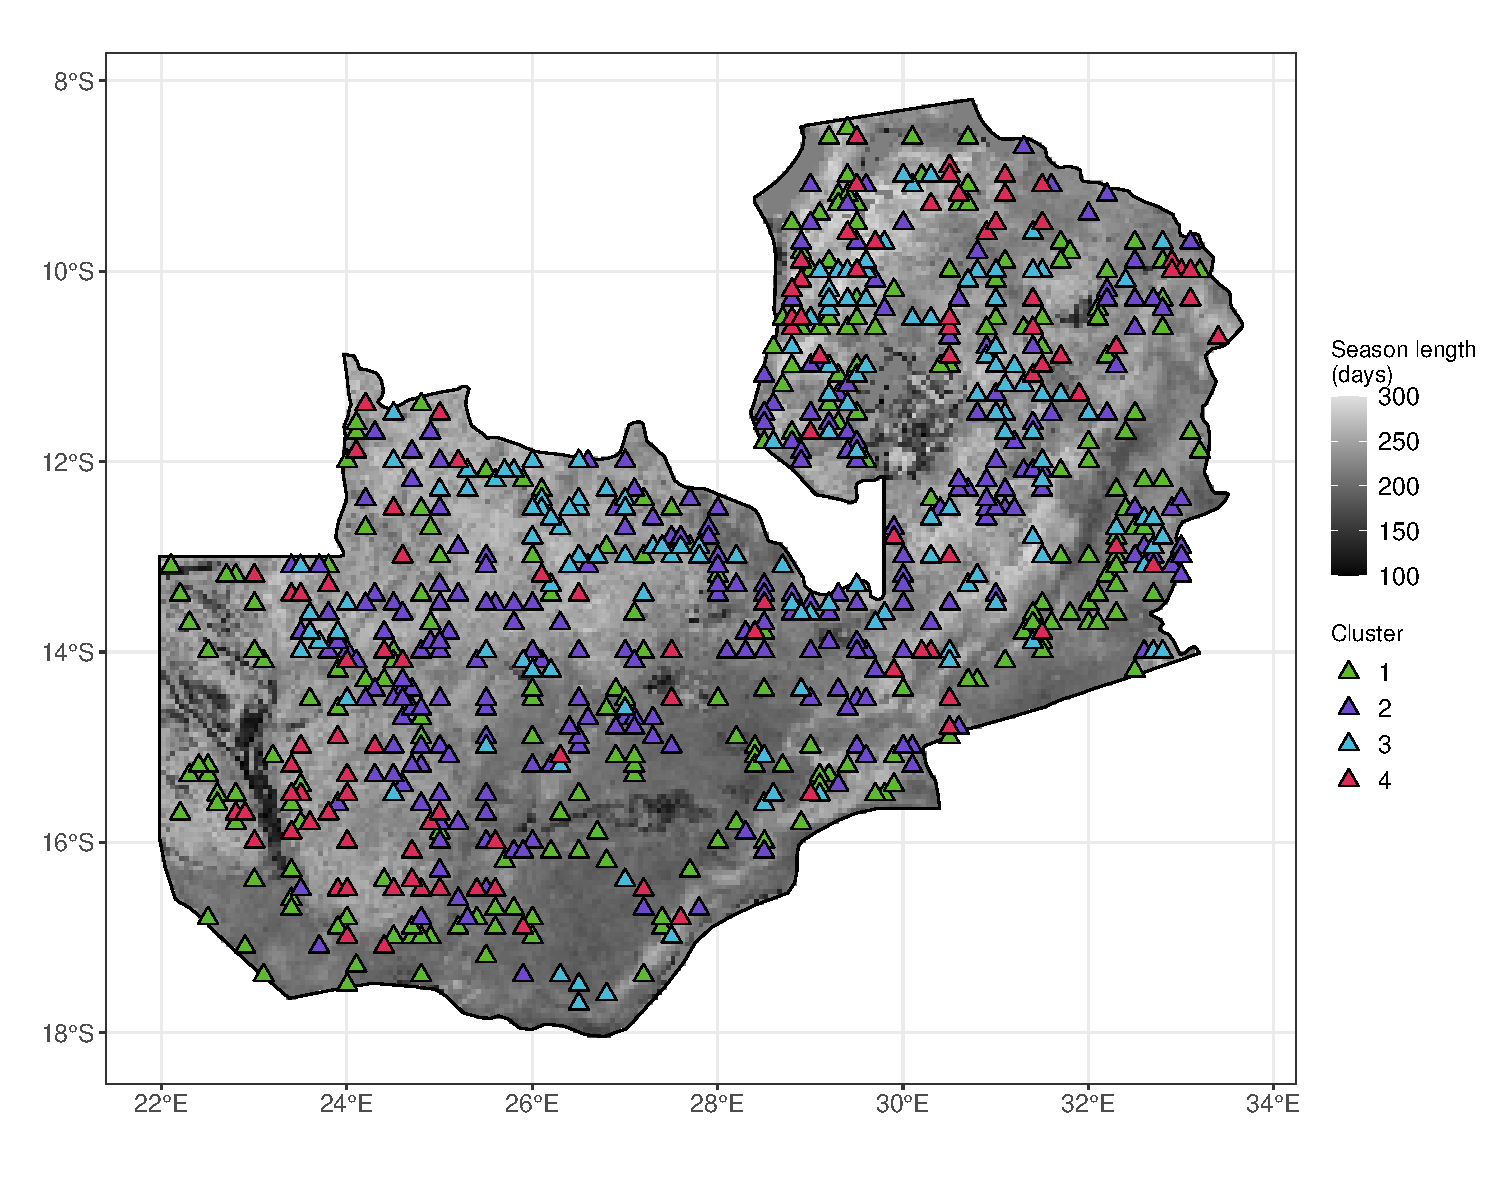
\includegraphics[width=0.8\textwidth]{plot_loc}
	\caption{Distribution of study sites within Zambia as triangles, each consisting of four plots. Sites are oloured according to vegetation compositional cluster as identifed by the PAM clustering algorithm on NSCA ordination axes of species abundance data. Zambia is shaded according to growing season length as estimated by the MODIS VIPPHEN-EVI2 product, at 0.05 degrees spatial resolution \citep{VIPPHEN}.}
	\label{plot_loc}
\end{figure}

\begin{figure}[h]
\centering
	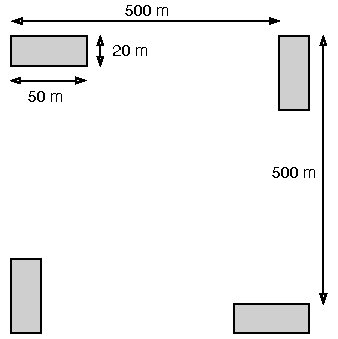
\includegraphics[width=0.5\textwidth]{schematic}
	\caption{Schematic diagram of plot layout within a site. Each 20x50 m (0.2 ha) plot is shaded grey. The site centre is denoted by a circle. Note that the plot dimensions are not to scale.}
	\label{schematic}
\end{figure}

Within each plot, the species of all trees with at least one stem $\geq$\stemSize{} cm DBH were recorded. Plot data was aggregated to the site level for analyses to avoid pseudo-replication caused by the more spatially coarse phenology data. Tree species composition varied little among the four plots within a site, and were treated as representative of the woodland in the local area. Using the Bray-Curtis dissimilarity index of species abundance data, we calculated that the mean pairwise compositional distance between plots within a site was lower than the mean compositional distance across all pairs of plots in \plotDistPer{}\% of cases. 

To quantify phenology at each site, we used the MODIS MOD13Q1 satellite data product at 250 m resolution \citep{MOD13Q1}. The MOD13Q1 product provides an Enhanced Vegetation Index (EVI) time series at 16 day intervals. EVI is widely used as a measure of vegetation growth, as an improvement to NDVI (Normalised Differential Vegetation Index), which tends to saturate at higher values. EVI is well-correlated with gross primary productivity and so can act as a suitable proxy \citep{}. We used all scenes from January 2015 to August 2020 with less than 20\% cloud cover covering the study area. All sites were determined to have a single annual growth season according to the MODIS VIPPHEN product \citep{}, which assigns pixels (0.05\textdegree, 5.55 km at equator) up to three growth seasons per year. We stacked yearly data between 2015 and 2020 and fit a General Additive Model (GAM) to produce an average EVI curve. We estimated the start and end of the growing season using the first derivative of the GAM. We identified the start of the growing season as the day where the slope of the curve first exceeds a slope of \modisSLC{}, which is maintained or exceeded for 10 or more days and the end of the growing season as the last day where the slope of the curve falls below -\modisSLC{}, which has been maintained for 10 or more days. We estimated the length of the growing season as the number of days between the start and end of the growing season defined as above. We estimated the greening rate as the slope of a linear model across EVI values between the start of the growing season and the point at which the slope of increase fell below \modisSLC{}. Similarly the senescence rate was estimated as the slope of a linear model between the point where the slope of decrease fell below -\modisSLC{} and the end of the growing season \autoref{ts_example}.

Precipitation data was gathered using the ``GPM IMERG Final Precipitation L3 1 day V06'' dataset, which has a pixel size of 0.1\textdegree (11.1 km at the equator) \citep{GPM}, between 2015 and 2020. Daily total precipitation was separated into two periods: precipitation during the growing season (growing season precipitation), and precipitation in the 90 day period before the onset of the growing season (dry season precipitation). Similar to estimation of the growing season, the rainy season was defined using the first derivative of a GAM to create a curve for each site using stacked yearly precipitation data. The slope coefficient used to identify the start and end of the rainy season was \trmmSLC{}. Mean diurnal temperature range (Diurnal $\delta$T) was calculated as the mean of monthly temperature range from the WorldClim database, using the BioClim variables, with a pixel size of 30 arc seconds (926 m at the equator) \citep{Fick2017}. averaged across all years of available data (1970-2000).

\begin{figure}[h]
\centering
	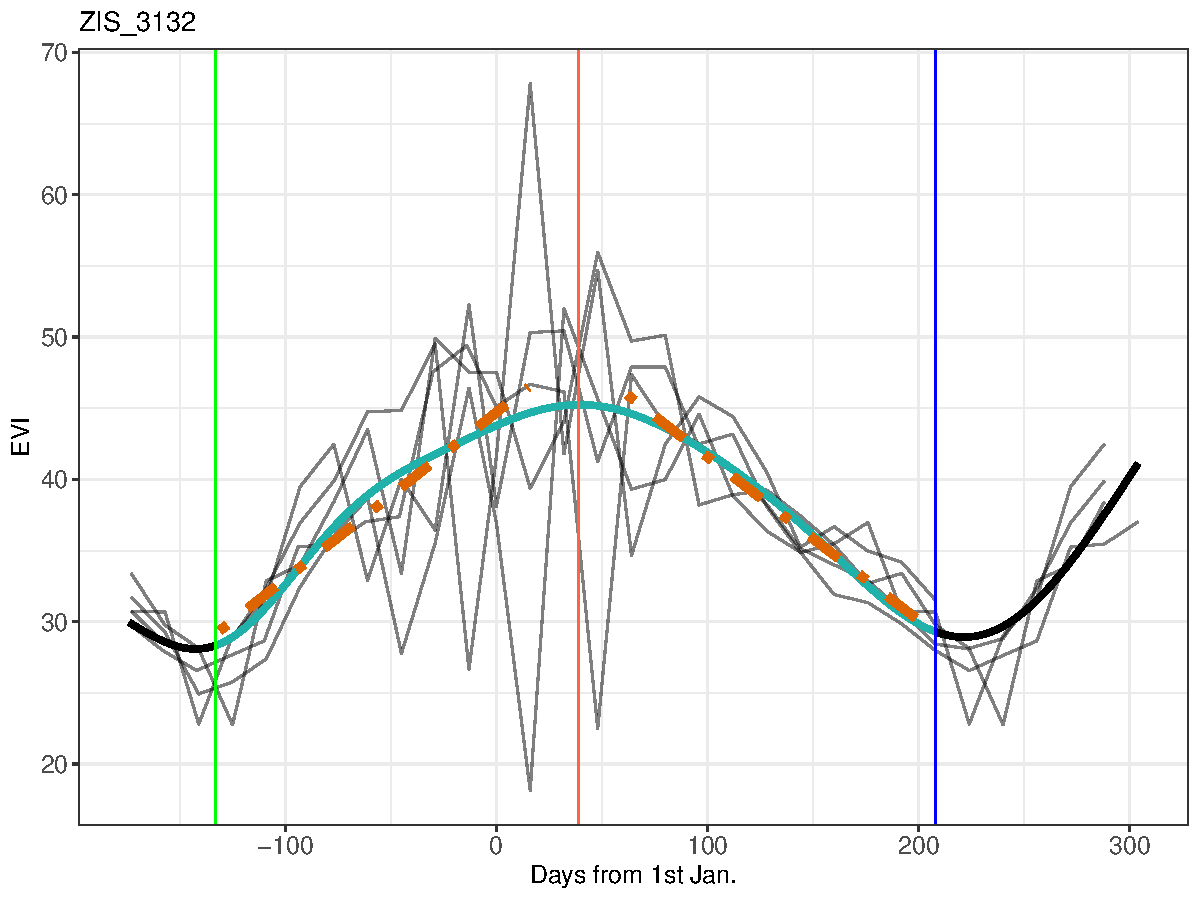
\includegraphics[width=0.8\textwidth]{ts_example}
	\caption{Example EVI time series, demonstrating the metrics derived from it. Thin black lines show the raw EVI time series, with one line for each annual growth season. The thick black line shows the GAM fit. The thin blue lines show the minima which bound the growing season. The red line shows the maximum EVI value reached within the growing season. The shaded cyan area of the GAM fit shows the growing season, as defined by the first derivative of the GAM curve. The two orange dashed lines are linear regressions predicting the greening rate and senescence rate at the start and end of the growing season, respectively. Note that while the raw EVI time series fluctuate greatly around the middle of the growing season, mostly due to cloud cover, the GAM fit effectively smooths this variation to estimate the average EVI during the mid-season period.}
	\label{ts_example}
\end{figure}

\subsection{Data analysis}

To quantify variation in tree species composition we used a Non-Symmetric Correspondence Analysis (NSCA), based on tree species abundance per site, with four axes (Inertia = \nscaInertia{}), using the \texttt{ade4} R package \citep{ade4}. The first 4 axes of the NSCA explained nscaPer{} of the variation in species composition among sites according to eigenvalue analysis. We performed clustering on the NSCA axes, using the PAM (Partitioning Around Medoids) algorithm available in the \texttt{cluster} R package \citep{cluster}. We identified four compositional groups based on this analysis which were used as random effects in statistical models. \todo{More technical detail on NSCA procedure}

We specified multivariate linear models to assess the role of tree species diversity on each of the chosen phenological metrics. We defined tree species diversity using both species richness and abundance evenness as separate independent variables. Abundance evenness was calculated as the Shannon Equitability index ($E_{H'}$) \citep{Smith1996} was calculated as the ratio of the Shannon diversity index to the natural log of species richness. We defined a maximal model structure including tree species richness, abundance evenness, the interaction of species richness and vegetation type, and climatic variables shown by previous studies to strongly influence phenology. The quality of the maximal model was compared to models with different subsets of independent variables using the model log likelihood, AIC (Akaike Information Criteria), BIC (Bayesian Information Criteria), and adjusted R\textsuperscript{2} values for each model. For each phenological metric, the best model according to the model quality statistics is reported in the results. All models were fitted using Maximum Likelihood to allow comparison of models \citep{}. Independent variables in each model were transformed to achieve normality where necessary and standardised to Z-scores prior to modelling to allow comparison of slope coefficients within a given model. All statistical analyses were conducted in R version 4.0.2 \citep{R2020}.

\section{Results}

Model selection showed that richness and evenness are important determinants of each phenological metric, across vegetation types \autoref{mod_slopes}. Models predicting rainy season - growing season lags included only species and richness. It is striking that in models for green-up lag and season length, species richness and evenness had contrasting effects on these phenological metrics. Species richness increased the green-up lag time and increased season length, while evenness had the opposite effect.

Against expectations, tree species richness and evenness had negative effects on cumulative EVI, while wet season precipitation had a positive effect and diurnal temperature range had a negative effect, as expected. Despite this, species richness had a positive effect on season length.

Model estimates for both greening rate were poorly constrained, with wide confidence intervals on model coefficients which overlapped zero, indicating that other unmeasured drivers had important influence over these variables. The model for greening rate explained <0.001\% of variance in the response variable. As expected, greening rate was negatively affected by species richness and abundance evenness. A higher species richness led to a slower rate of greening. 

Interestingly, the best models for start of season and end of season lag time included only species richness and evenness as fixed effects. An increase in species richness led to an increase in the negative lag between the start of the growing season and the start of the rainy season, while the opposite was true for the lag between the end of the growing season and the end of the rainy season. 

For all phenological metrics, models including species richness and evenness were of better quality than those containing only climatic variables.  

The slope of the relationship between species richness and phenological metrics varied among vegetation types, but largely maintained the same direction. Only in greening rate, senescencerate, and season length did vegetation types have differing slope estimates.

% latex table generated in R 4.0.2 by xtable 1.8-4 package
% Wed Oct 28 12:24:01 2020
\begin{table}[H]
\centering
\begin{tabular}{ccc}
  \hline
Cluster & Species & Indicator value \\ 
  \hline
1 & \textit{Pterocarpus angolensis} & 0.294 \\ 
  1 & \textit{Diplorhynchus condylocarpon} & 0.265 \\ 
  1 & \textit{Brachystegia spiciformis} & 0.252 \\ 
   \hline
2 & \textit{Brachystegia boehmii} & 0.795 \\ 
  2 & \textit{Psuedolachnostylis maprouneifolia} & 0.240 \\ 
  2 & \textit{Uapaca kirkiana} & 0.224 \\ 
   \hline
3 & \textit{Julbernardia paniculata} & 0.717 \\ 
  3 & \textit{Psuedolachnostylis maprouneifolia} & 0.272 \\ 
  3 & \textit{Diplorhynchus condylocarpon} & 0.228 \\ 
  \end{tabular}
\caption{Legendre indicator species analysis for the four vegetation type clusters identified by the PAM algorithm.} 
\label{indval}
\end{table}



% latex table generated in R 4.0.2 by xtable 1.8-4 package
% Sat Oct 31 12:21:16 2020
\begin{table}[H]
\centering
\begin{tabular}{rcccc}
  \hline
Response & $\delta$AIC & $\delta$BIC & R\textsuperscript{2}\textsubscript{adj} & $\delta$logLik \\ 
  \hline
Cumulative EVI & 43.1 & 34.0 & 0.34 & -23.54 \\ 
  Season length & 25.9 & 21.4 & 0.17 & -13.97 \\ 
  Green-up rate & 8.1 & 3.6 & 0.10 & -5.07 \\ 
  Senescence rate & 10.1 & 1.0 & 0.03 & -7.04 \\ 
  Green-up lag & 67.7 & 63.2 & 0.26 & -34.87 \\ 
  Senescence lag & 7.8 & 7.8 & 0.02 & -3.88 \\ 
   \hline
\end{tabular}
\caption{Model fit statistics for each phenological metric.} 
\label{mod_stat}
\end{table}

 

\begin{figure}[h]
\centering
	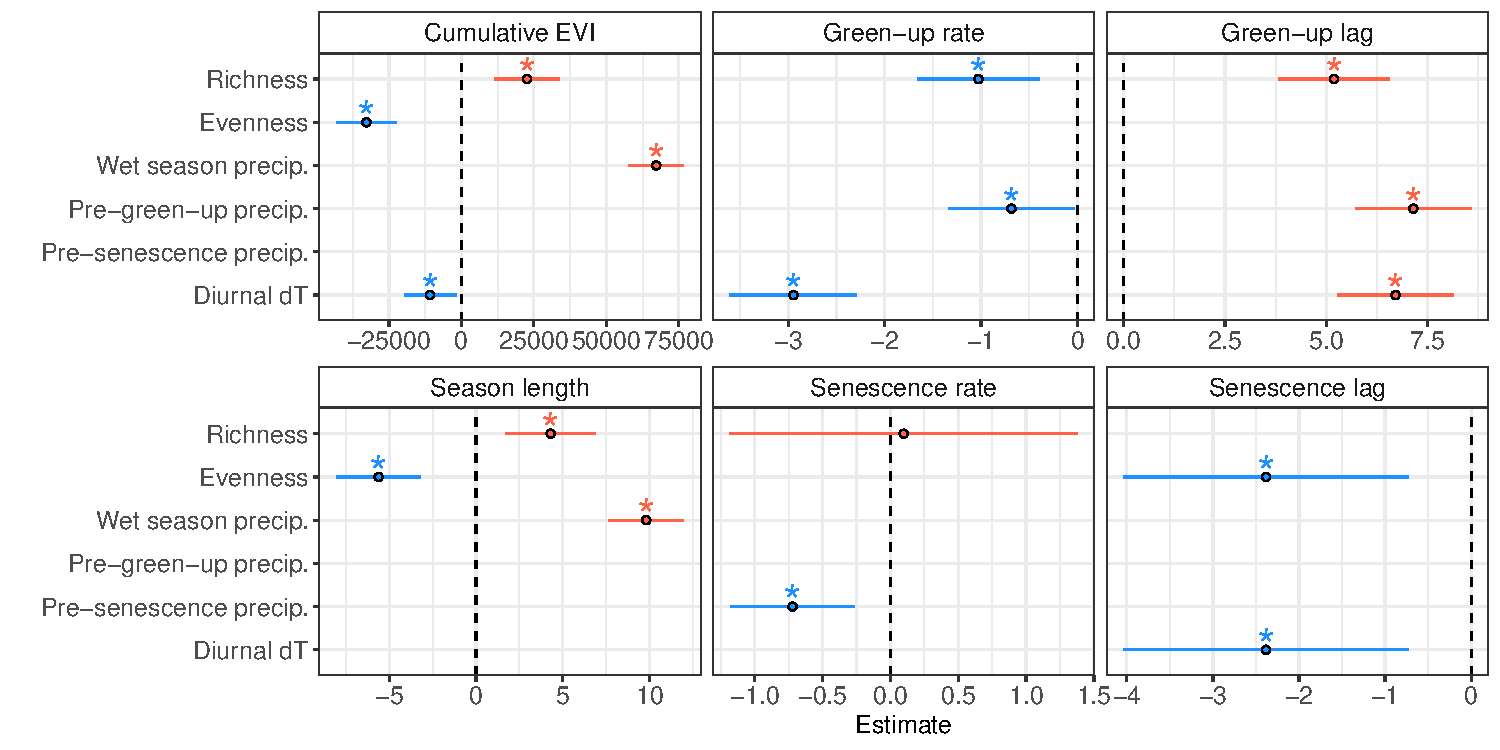
\includegraphics[width=\textwidth]{mod_slopes.pdf}
	\caption{Standardized slope coefficients for each best model of a phenological metric. Slope estimates are $\pm$1 standard error. Slope estimates where the interval (standard error) does not overlap zero are considered to be significant effects.}
	\label{mod_slopes}
\end{figure}

\begin{figure}[h]
\centering
	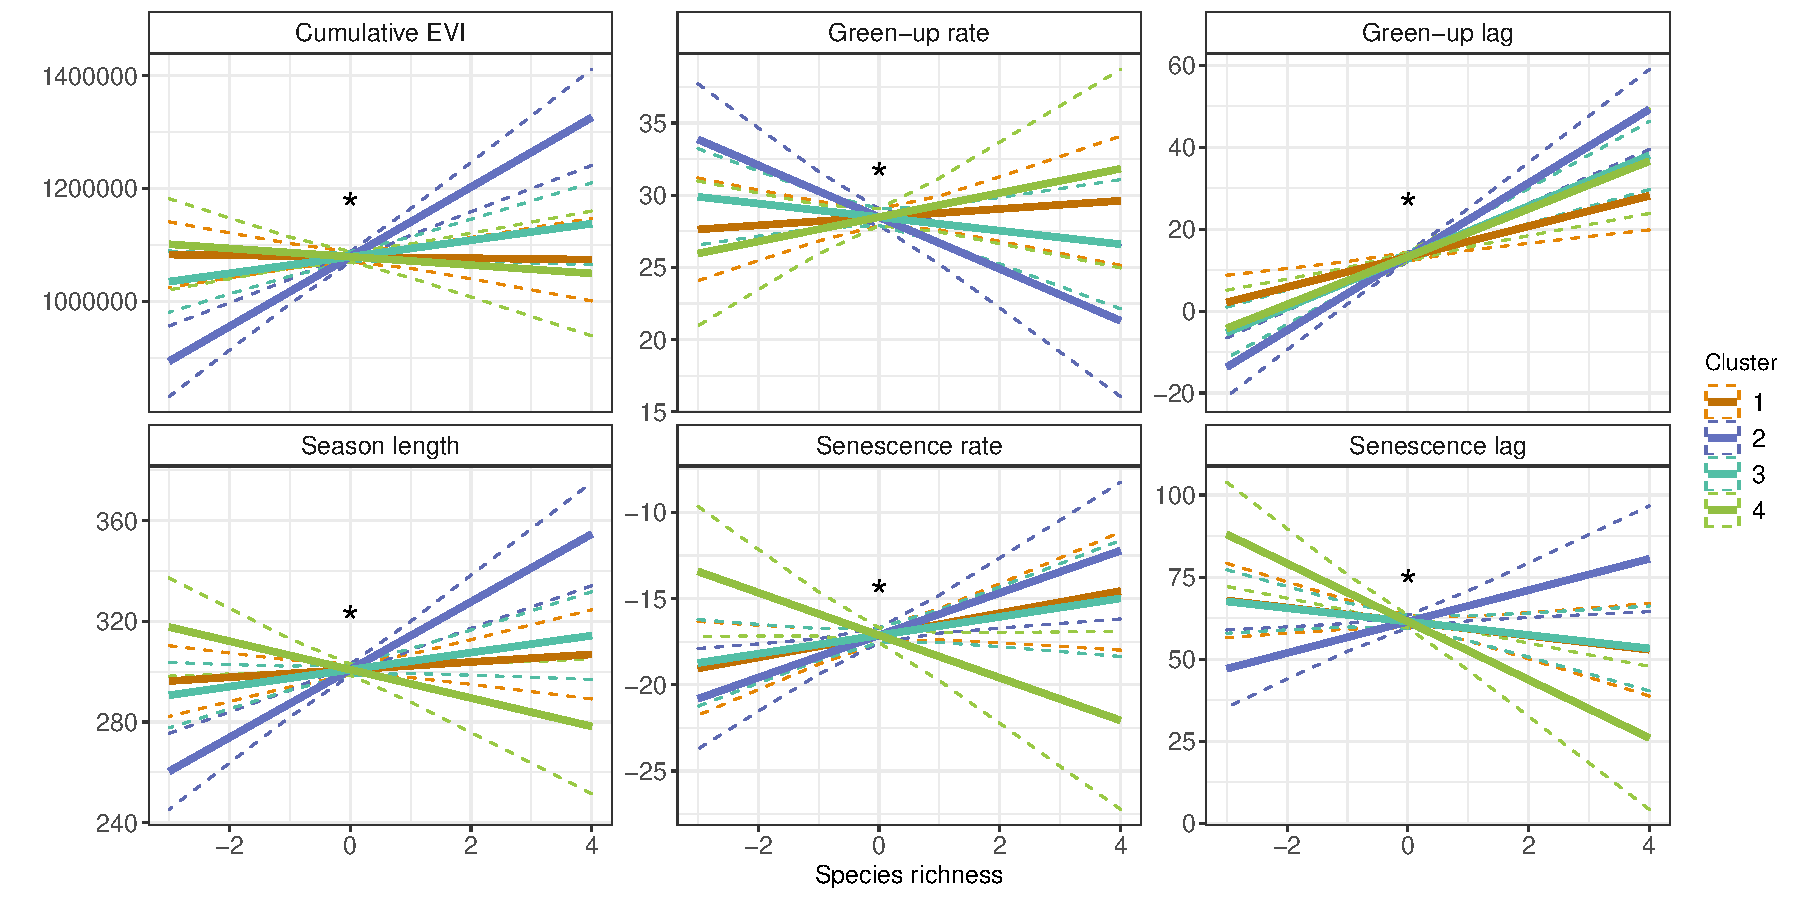
\includegraphics[width=\textwidth]{mod_marg.pdf}
	\caption{Marginal effects of tree species richness on each of the phenological metrics, for each vegetation type, using the best model for each phenological metric.}
	\label{mod_marg}
\end{figure}

\begin{figure}[h]
\centering
	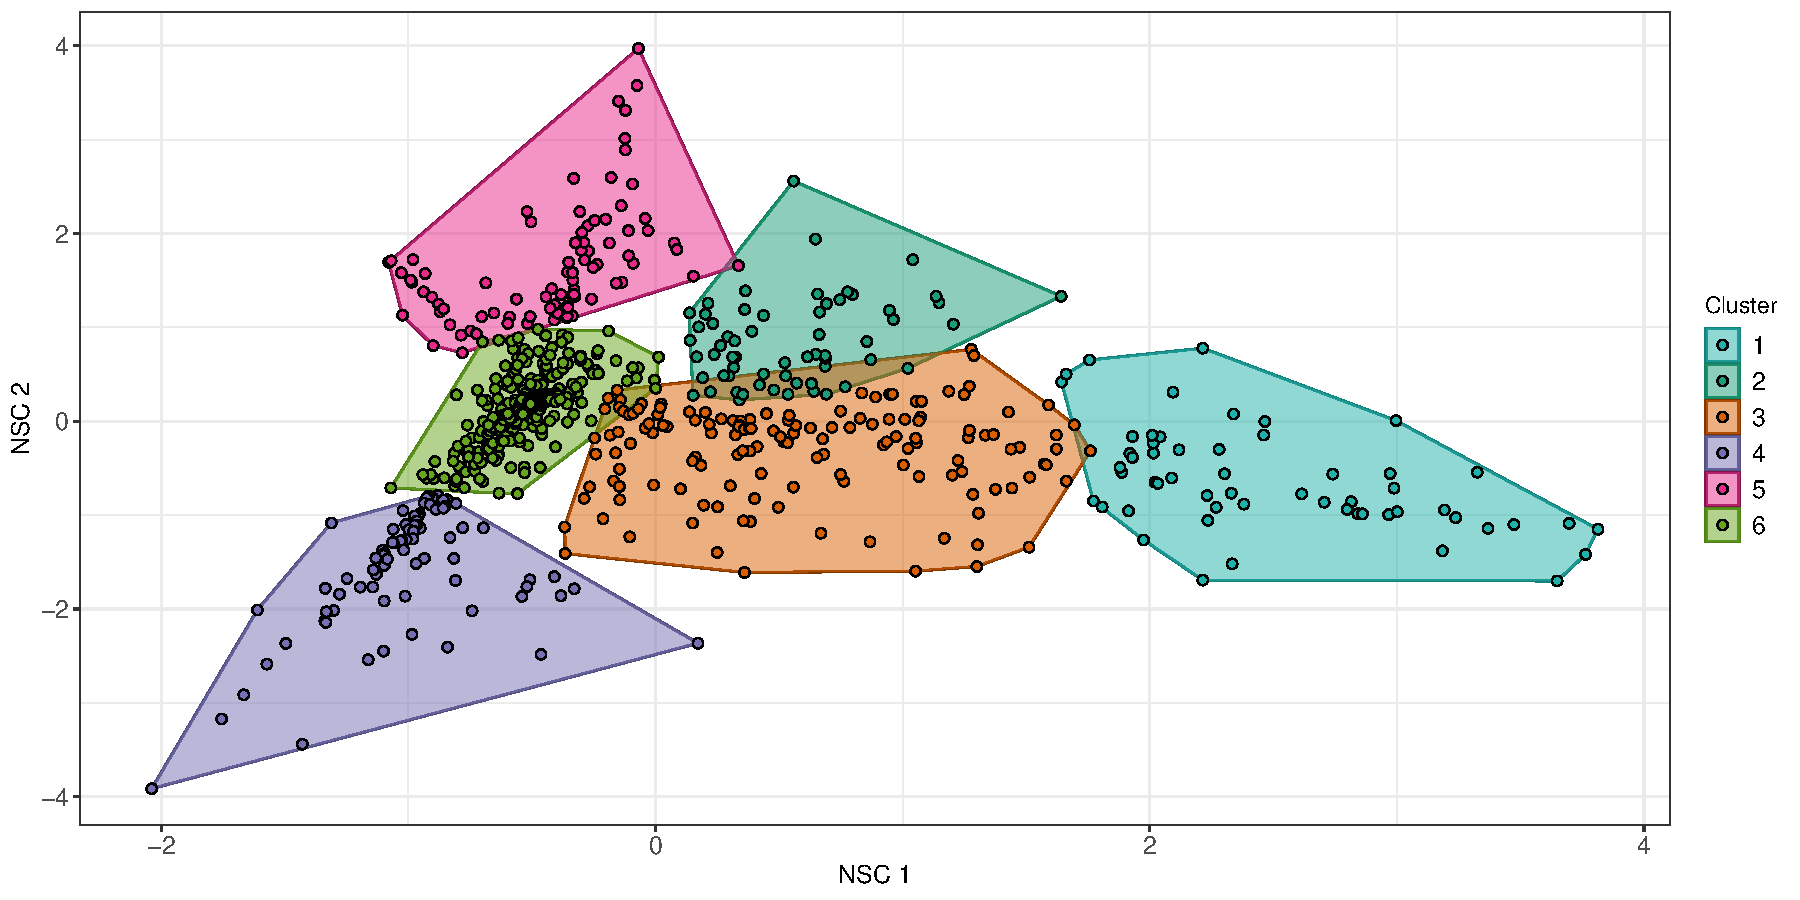
\includegraphics[width=\textwidth]{nsca.pdf}
	\caption{Plot scores of the (A) first and second, and (B) third and fourth axes of the Non-Symmetric Correspondence Analysis of tree species composition. Points are coloured according to clusters defined by the PAM algorithm on the NSCA ordination axes, along with a convex hull encompassing 95\% of the points in each cluster.}
	\label{nsca}
\end{figure}

\begin{figure}[h]
\centering
	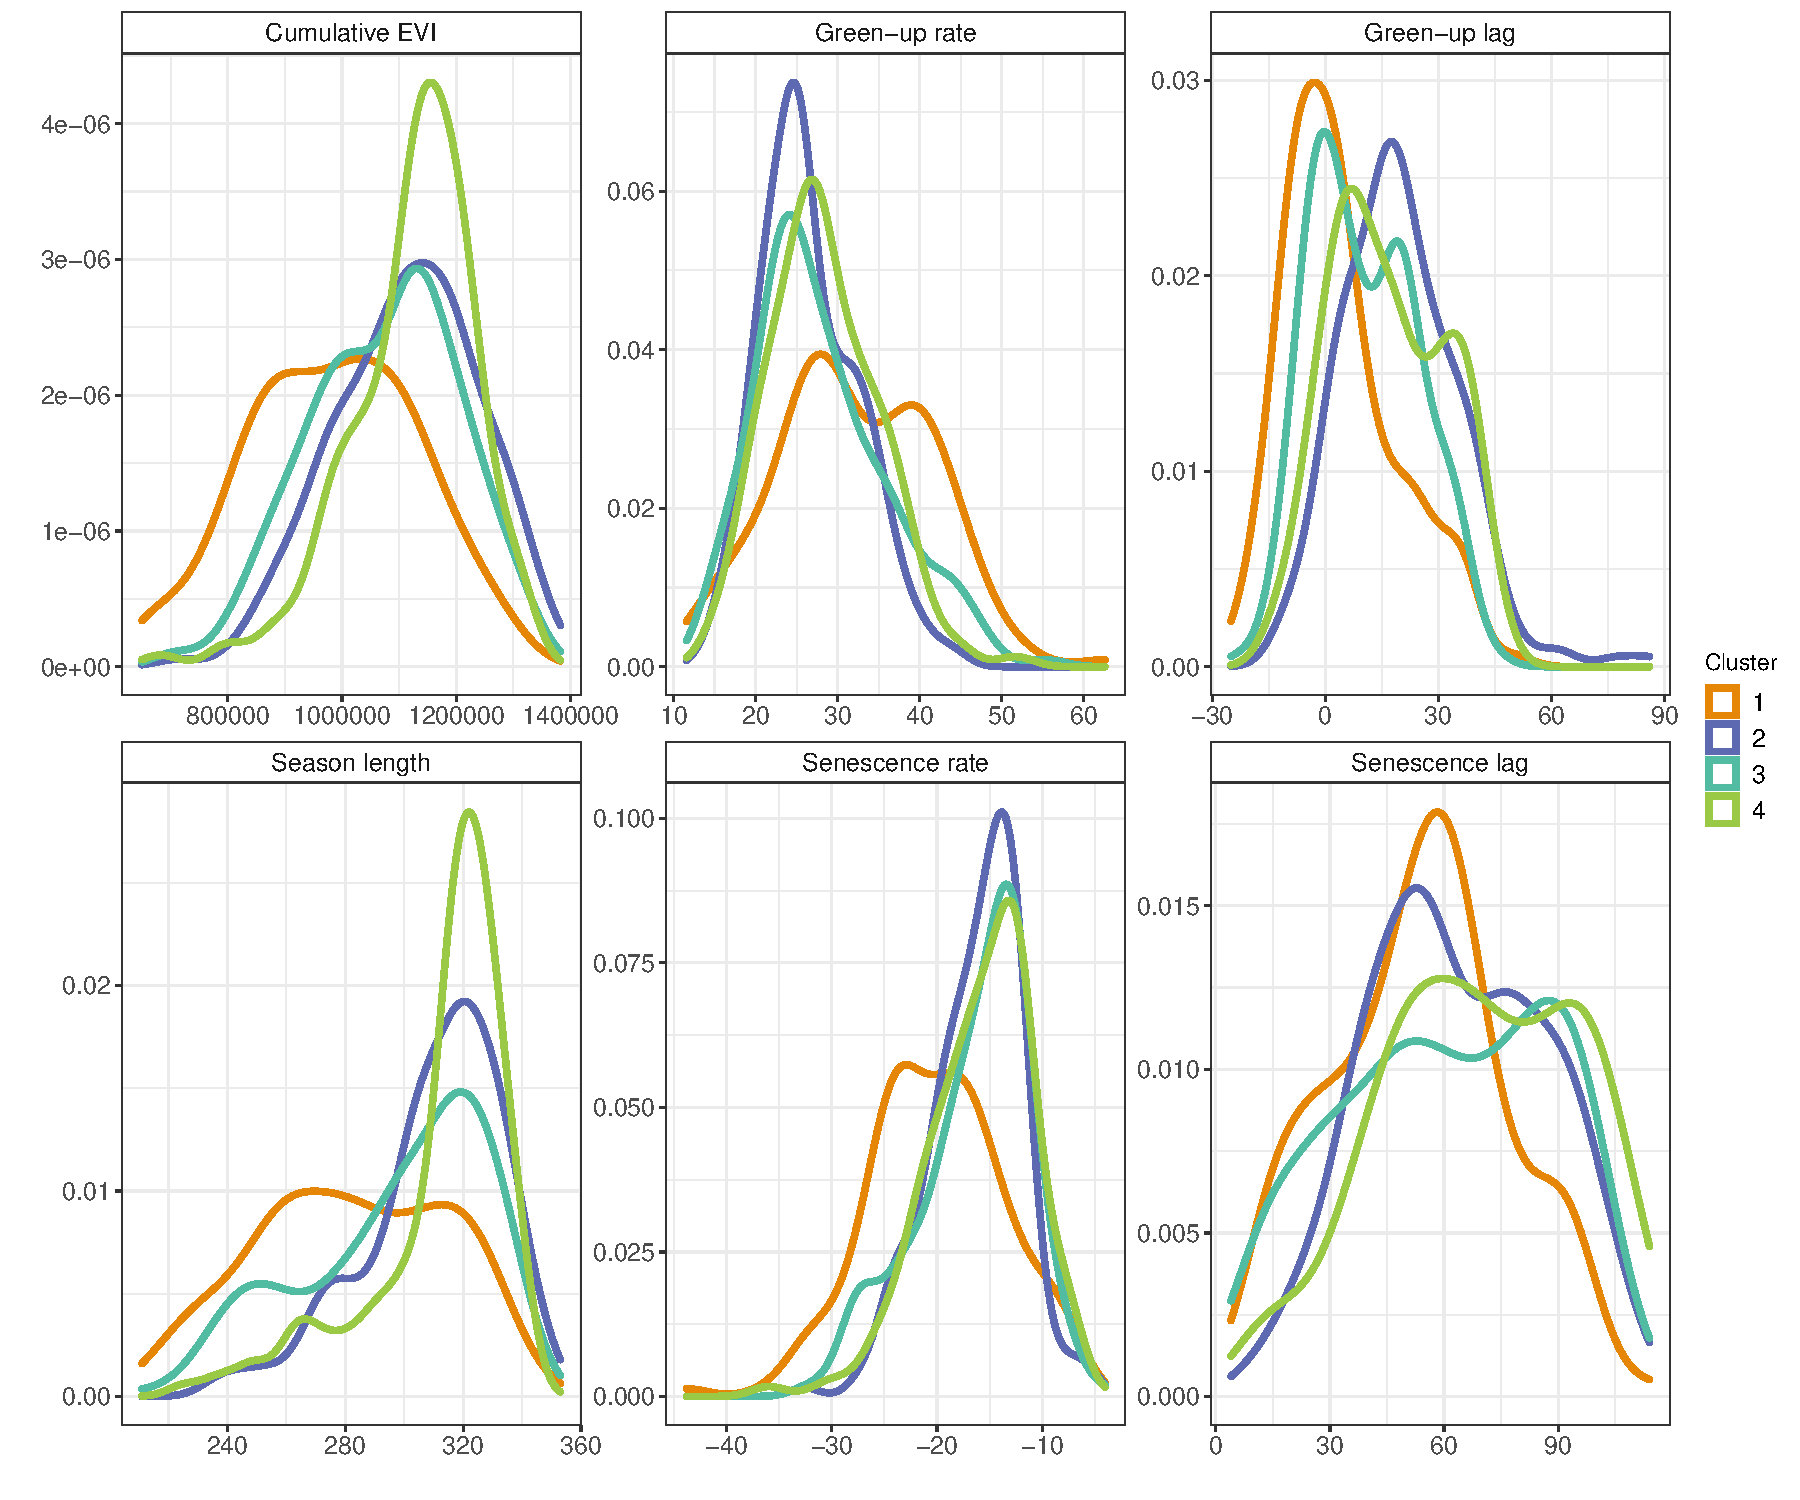
\includegraphics[width=\textwidth]{phen_dens_clust}
	\caption{}
	\label{phen_dens_clust}
\end{figure}

\section{Discussion}

The ability for us now nearing to be able to remotely sense tree species diversity allows us to make more tailored models of the carbon cycle which incorporate not only climatic factors, but also biotic factors which govern productivity. We therefore need to understand how species composition and biodiversity metrics affect land-surface phenology. 

\section{Conclusion}

\printbibliography

\section{Supplementary material}

% latex table generated in R 4.0.2 by xtable 1.8-4 package
% Tue Oct 27 08:49:06 2020
\begin{table}[ht]
\centering
\begin{tabular}{cccccrrrr}
  \hline
Rank & Precipitation & Diurnal dT & Evenness & Richness & logLik & AIC & $\Delta{}IC$ & $W_{i}$ \\ 
  \hline
1 & \checkmark & \checkmark & \checkmark & \checkmark & -5933 & 11885 & 0.00 & 0.333 \\ 
  2 & \checkmark & \checkmark & \checkmark & \checkmark & -5935 & 11885 & 0.21 & 0.299 \\ 
  3 & \checkmark & \checkmark &  & \checkmark & -5937 & 11887 & 2.08 & 0.118 \\ 
  4 & \checkmark & \checkmark & \checkmark &  & -5937 & 11887 & 2.14 & 0.115 \\ 
  5 & \checkmark & \checkmark &  & \checkmark & -5935 & 11887 & 2.31 & 0.105 \\ 
  6 & \checkmark & \checkmark &  &  & -5940 & 11890 & 4.77 & 0.031 \\ 
  7 &  & \checkmark & \checkmark &  & -5947 & 11904 & 18.38 & 0.000 \\ 
  8 &  & \checkmark &  &  & -5948 & 11905 & 20.15 & 0.000 \\ 
  9 &  & \checkmark & \checkmark & \checkmark & -5946 & 11905 & 20.26 & 0.000 \\ 
  10 &  & \checkmark & \checkmark & \checkmark & -5945 & 11906 & 20.99 & 0.000 \\ 
   \hline
\end{tabular}
\caption{Cumulative EVI model selection candidate models, with fit statistics.} 
\label{mod_sel_cum_vi}
\end{table}

% latex table generated in R 4.0.2 by xtable 1.8-4 package
% Tue Oct 27 08:49:07 2020
\begin{table}[ht]
\centering
\begin{tabular}{cccccrrrr}
  \hline
Rank & Precipitation & Diurnal dT & Evenness & Richness & logLik & AIC & $\Delta{}IC$ & $W_{i}$ \\ 
  \hline
1 & \checkmark & \checkmark &  & \checkmark & -3041 & 6094 & 0.00 & 0.346 \\ 
  2 & \checkmark & \checkmark &  & \checkmark & -3039 & 6094 & 0.05 & 0.338 \\ 
  3 & \checkmark & \checkmark & \checkmark & \checkmark & -3039 & 6096 & 1.53 & 0.161 \\ 
  4 & \checkmark & \checkmark & \checkmark & \checkmark & -3041 & 6096 & 1.63 & 0.153 \\ 
  5 &  & \checkmark &  & \checkmark & -3046 & 6107 & 13.27 & 0.000 \\ 
  6 &  & \checkmark &  & \checkmark & -3048 & 6107 & 13.28 & 0.000 \\ 
  7 &  & \checkmark & \checkmark & \checkmark & -3046 & 6109 & 14.93 & 0.000 \\ 
  8 &  & \checkmark & \checkmark & \checkmark & -3048 & 6109 & 15.04 & 0.000 \\ 
  9 & \checkmark & \checkmark &  &  & -3059 & 6128 & 34.02 & 0.000 \\ 
  10 & \checkmark & \checkmark & \checkmark &  & -3058 & 6129 & 34.77 & 0.000 \\ 
   \hline
\end{tabular}
\caption{Senescence lag model selection candidate models, with fit statistics.} 
\label{mod_sel_end_lag}
\end{table}

% latex table generated in R 4.0.2 by xtable 1.8-4 package
% Tue Oct 27 08:49:07 2020
\begin{table}[ht]
\centering
\begin{tabular}{cccccrrrr}
  \hline
Rank & Precipitation & Diurnal dT & Evenness & Richness & logLik & AIC & $\Delta{}IC$ & $W_{i}$ \\ 
  \hline
1 & \checkmark & \checkmark &  & \checkmark & 881 & -1751 & 0.00 & 0.369 \\ 
  2 & \checkmark & \checkmark & \checkmark & \checkmark & 881 & -1749 & 1.35 & 0.188 \\ 
  3 & \checkmark & \checkmark &  & \checkmark & 882 & -1749 & 1.91 & 0.142 \\ 
  4 &  & \checkmark &  & \checkmark & 879 & -1748 & 2.88 & 0.087 \\ 
  5 & \checkmark & \checkmark & \checkmark & \checkmark & 883 & -1748 & 3.05 & 0.080 \\ 
  6 &  & \checkmark & \checkmark & \checkmark & 879 & -1746 & 4.45 & 0.040 \\ 
  7 &  & \checkmark &  & \checkmark & 880 & -1746 & 4.89 & 0.032 \\ 
  8 & \checkmark & \checkmark &  &  & 877 & -1745 & 5.46 & 0.024 \\ 
  9 & \checkmark & \checkmark & \checkmark &  & 878 & -1744 & 6.28 & 0.016 \\ 
  10 &  & \checkmark & \checkmark & \checkmark & 880 & -1744 & 6.29 & 0.016 \\ 
   \hline
\end{tabular}
\caption{Green-up rate model selection candidate models, with fit statistics.} 
\label{mod_sel_s1_green_rate}
\end{table}

% latex table generated in R 4.0.2 by xtable 1.8-4 package
% Tue Oct 27 08:49:07 2020
\begin{table}[ht]
\centering
\begin{tabular}{cccccrrrr}
  \hline
Rank & Precipitation & Diurnal dT & Evenness & Richness & logLik & AIC & $\Delta{}IC$ & $W_{i}$ \\ 
  \hline
1 & \checkmark &  & \checkmark & \checkmark & -2966 & 5945 & 0.00 & 0.448 \\ 
  2 & \checkmark & \checkmark & \checkmark & \checkmark & -2966 & 5946 & 1.43 & 0.220 \\ 
  3 & \checkmark &  & \checkmark & \checkmark & -2965 & 5947 & 2.08 & 0.158 \\ 
  4 & \checkmark & \checkmark & \checkmark & \checkmark & -2965 & 5948 & 3.53 & 0.077 \\ 
  5 & \checkmark &  & \checkmark &  & -2969 & 5949 & 3.96 & 0.062 \\ 
  6 & \checkmark & \checkmark & \checkmark &  & -2969 & 5950 & 5.69 & 0.026 \\ 
  7 & \checkmark &  &  & \checkmark & -2972 & 5954 & 9.49 & 0.004 \\ 
  8 & \checkmark & \checkmark &  & \checkmark & -2971 & 5955 & 10.67 & 0.002 \\ 
  9 & \checkmark &  &  & \checkmark & -2971 & 5957 & 11.90 & 0.001 \\ 
  10 & \checkmark &  &  &  & -2974 & 5957 & 11.92 & 0.001 \\ 
   \hline
\end{tabular}
\caption{Season length model selection candidate models, with fit statistics.} 
\label{mod_sel_s1_length}
\end{table}

% latex table generated in R 4.0.2 by xtable 1.8-4 package
% Tue Oct 27 08:49:07 2020
\begin{table}[ht]
\centering
\begin{tabular}{cccccrrrr}
  \hline
Rank & Precipitation & Diurnal dT & Evenness & Richness & logLik & AIC & $\Delta{}IC$ & $W_{i}$ \\ 
  \hline
1 & \checkmark & \checkmark &  & \checkmark & 1245 & -2474 & 0.00 & 0.449 \\ 
  2 & \checkmark &  &  & \checkmark & 1243 & -2472 & 1.70 & 0.192 \\ 
  3 & \checkmark & \checkmark & \checkmark & \checkmark & 1245 & -2472 & 1.80 & 0.182 \\ 
  4 & \checkmark &  & \checkmark & \checkmark & 1243 & -2470 & 3.56 & 0.076 \\ 
  5 & \checkmark & \checkmark &  & \checkmark & 1240 & -2469 & 4.63 & 0.044 \\ 
  6 & \checkmark &  &  & \checkmark & 1239 & -2468 & 5.98 & 0.023 \\ 
  7 & \checkmark & \checkmark & \checkmark & \checkmark & 1240 & -2467 & 6.51 & 0.017 \\ 
  8 & \checkmark &  & \checkmark & \checkmark & 1239 & -2466 & 7.92 & 0.009 \\ 
  9 & \checkmark &  &  &  & 1236 & -2464 & 10.04 & 0.003 \\ 
  10 & \checkmark & \checkmark &  &  & 1237 & -2464 & 10.16 & 0.003 \\ 
   \hline
\end{tabular}
\caption{Senescence rate model selection candidate models, with fit statistics.} 
\label{mod_sel_s1_senes_rate}
\end{table}

% latex table generated in R 4.0.2 by xtable 1.8-4 package
% Tue Oct 27 08:49:07 2020
\begin{table}[ht]
\centering
\begin{tabular}{cccccrrrr}
  \hline
Rank & Precipitation & Diurnal dT & Evenness & Richness & logLik & AIC & $\Delta{}IC$ & $W_{i}$ \\ 
  \hline
1 & \checkmark & \checkmark & \checkmark & \checkmark & -3074 & 6167 & 0.00 & 0.563 \\ 
  2 & \checkmark & \checkmark &  & \checkmark & -3076 & 6168 & 1.63 & 0.249 \\ 
  3 & \checkmark & \checkmark & \checkmark & \checkmark & -3077 & 6169 & 2.85 & 0.135 \\ 
  4 & \checkmark & \checkmark &  & \checkmark & -3079 & 6171 & 4.72 & 0.053 \\ 
  5 & \checkmark & \checkmark &  &  & -3102 & 6215 & 48.86 & 0.000 \\ 
  6 & \checkmark & \checkmark & \checkmark &  & -3102 & 6216 & 49.48 & 0.000 \\ 
  7 &  & \checkmark & \checkmark & \checkmark & -3130 & 6273 & 106.35 & 0.000 \\ 
  8 &  & \checkmark & \checkmark & \checkmark & -3128 & 6273 & 106.77 & 0.000 \\ 
  9 &  & \checkmark &  & \checkmark & -3133 & 6277 & 110.46 & 0.000 \\ 
  10 &  & \checkmark &  & \checkmark & -3131 & 6277 & 110.63 & 0.000 \\ 
   \hline
\end{tabular}
\caption{Green-up lag model selection candidate models, with fit statistics.} 
\label{mod_sel_start_lag}
\end{table}



\end{document}

